\chapter{Lý Thuyết}
\label{chap:background}
\graphicspath{{Chapter3/Figs/}}

\begin{chapabstract}
Đầu tiên, chương \ref{chap:background} trình bày các nền tảng lý thuyết được sử dụng trong đề tài, bao gồm các loại malware, PE file format và các kiến thức lý thuyết khác về học máy. Sau đó, các thước đo đánh giá và framework sử dụng cho thuật toán học máy đã được sử dụng trong việc implement thuật toán sẽ được giới thiệu.
\end{chapabstract}

\section{Malware Types}
\label{sec:malware}

Phân loại là cách tuyệt vời để hiểu rõ hơn về phần mềm độc hại. Một số loại phổ biến nhất bao gồm: adware, bots, rootkits, spyware, Trojan horses, viruses, and worms \cite{neil2012common}.

\subsection{Virus}

Virus là một dạng phần mềm độc hại có khả năng sao chép chính nó và lây lan sang các máy tính khác bằng cách đính kèm vào các ứng dụng khác nhau và thực thi khi người dùng khởi chạy một trong số đó. Virus cũng có thể lây lan qua các tài liệu, tệp kịch bản và lỗ hổng tập lệnh script (cross-site scripting vulnerabilities) trong các ứng dụng web. Một số ví dụ nổi tiếng của virus trong những năm qua là virus Concept, virus Chernobyl (còn được gọi là CIH), virus Anna Kournikova, Brain và RavMonE.exe.

\subsection{Worm}

Worm là một phần mềm độc lập sao chép mà không cần nhắm mục tiêu và lây nhiễm các tệp cụ thể. Hãy nghĩ về worm như các chương trình nhỏ tự sao chép bản thân và phá hủy dữ liệu. Nó thường nhắm vào các tập tin hệ điều hành và làm việc cho đến khi ổ đĩa trở nên trống rỗng. Một số ví dụ bao gồm Melissa, Morris, Mydoom, Sasser và Blaster.

\subsection{Trojan}

Trojan là một ứng dụng độc hại giả dạng bản thân để trông hữu ích và đánh lừa người dùng tải xuống và cài đặt. Trojan có thể cung cấp quyền truy cập từ xa vào một máy tính bị nhiễm để kẻ tấn công có thể lấy cắp dữ liệu, cài đặt thêm phần mềm độc hại, theo dõi hoạt động của người dùng, v.v. Các ví dụ đáng chú ý cũng bao gồm những con Trojan được phát triển bởi các cơ quan chính phủ Hoa Kỳ như FBI và NSA. Những cái tên như Magic Lantern, FinFisher, Netbus, Beast, Gh0st RAT, Clickbot.A, và Zeus đã trở thành lý do của kinh sự kinh hoàng. Tương tự  một trojan trên Android được phát hiện vào năm 2015, tên là Shedun, là một trong nhiều malware nhắm đến mục tiêu là thiết bị di động.

\subsection{Ransomware}

Ransomware, một trong những phần mềm độc hại nhất và liên tục xuất hiện, là một loại phần mềm độc hại thường giam giữ một hệ thống máy tính và yêu cầu một khoản tiền chuộc, ví dụ như chặn truy cập vào dữ liệu của nạn nhân hoặc đe dọa công khai nội dung của nó. Tệ hơn nữa, không có gì đảm bảo rằng việc thanh toán sẽ nhận được quyền truy cập vào dữ liệu hoặc ngăn không cho công khai dữ liệu nhạy cảm. Các ransomware nổi tiếng như Reveton, CryptoLocker, CryptoWall, và gần đây hơn, cuộc tấn công WannaCry năm 2017, đã gây ra không một lượng không nhỏ tổn hại \cite{chen2017automated}.

\subsection{Rootkit}

Rootkit là một tập hợp các phần mềm được thiết kế đặc biệt để cho phép phần mềm độc hại xâm nhập hệ thống của bạn và thu thập thông tin. Những công việc này ở chế độ nền để người dùng có thể không nhận thấy bất kỳ điều gì khác biệt. Nhưng bên trong môi trường, một rootkit sẽ cho phép một số loại phần mềm độc hại xâm nhập vào hệ thống. Rootkit đầu tiên có được danh tiếng trên Windows là NTRootkit vào năm 1999, nhưng phổ biến nhất là vụ bê bối Sony BMG copy protection rootkit scandal đã làm rung chuyển công ty trong năm 2005 \cite{bruce2005sony}.

\subsection{Adware}

Mặc dù phần mềm hỗ trợ quảng cáo (adware) hiện phổ biến hơn nhiều, adware đã được liên kết với phần mềm độc hại trong một thời gian dài. Trong khi phần mềm quảng cáo có thể tham chiếu đến bất kỳ ứng dụng nào được quảng cáo hỗ trợ, phần mềm quảng cáo độc hại thường hiển thị quảng cáo dưới dạng cửa sổ bật lên và ngăn cửa sổ không thể đóng. Đó có lẽ là phần mềm độc hại hiệu quả nhất và ít nguy hiểm nhất, được thiết kế với mục đích cụ thể là quảng bá quảng cáo trên máy tính của bạn.

\subsection{Bot}

Bots là các chương trình phần mềm được tạo ra để thực hiện các hoạt động cụ thể một cách tự động. Trong khi một số bot được tạo ra cho mục đích vô hại, nó ngày càng trở nên phổ biến để xem bot đang được sử dụng độc hại. Bots có thể được sử dụng trong botnet (tập hợp các máy được kiểm soát bởi các bên thứ ba) để thực hiện các tấn công từ chối dịch vụ phân tán, gửi spam và ăn cắp dữ liệu.

\section{PE File Format}
\label{sec:pe-file}

Định dạng tệp Portable Executable (PE) mô tả định dạng thực thi chiếm ưu thế cho hệ điều hành Microsoft Windows và bao gồm tệp thực thi, thư viện liên kết động (DLL) và tệp phông chữ FON. Định dạng này hiện được hỗ trợ trên Intel, AMD và các biến thể của kiến trúc bộ lệnh ARM.

Tệp PE bao gồm một số header và section mô tả dynamic linker biết cách ánh xạ tệp vào bộ nhớ. Một tệp thực thi bao gồm một số vùng khác nhau, mỗi vùng đòi hỏi sự bảo vệ bộ nhớ khác nhau; do đó, bắt đầu của mỗi phần phải được căn chỉnh với một khung trang. Thông thường, các header bao gồm Common Object File Format (COFF) file header chứa các thông tin cần thiết như machine type, file type (DLL, EXE, OBJ), số lượng sections, số lượng symbols, v.v. Optional header xác định linker version, kích thước của code, kích thước của initialized data và uninitialized data, entry point address, v.v. Các data directory nằm optional header cung cấp con trỏ đến section chứa nó. Những section này bao gồm tables for exports, imports, resources, exceptions, debug information, certificate information, và relocation tables. Do đó, định dạng PE cung cấp một bản tổng hợp các thông tin hữu ích của một tệp thực thi \cite{shafiq2009pe}. 

\begin{figure}[H] 
\centering    
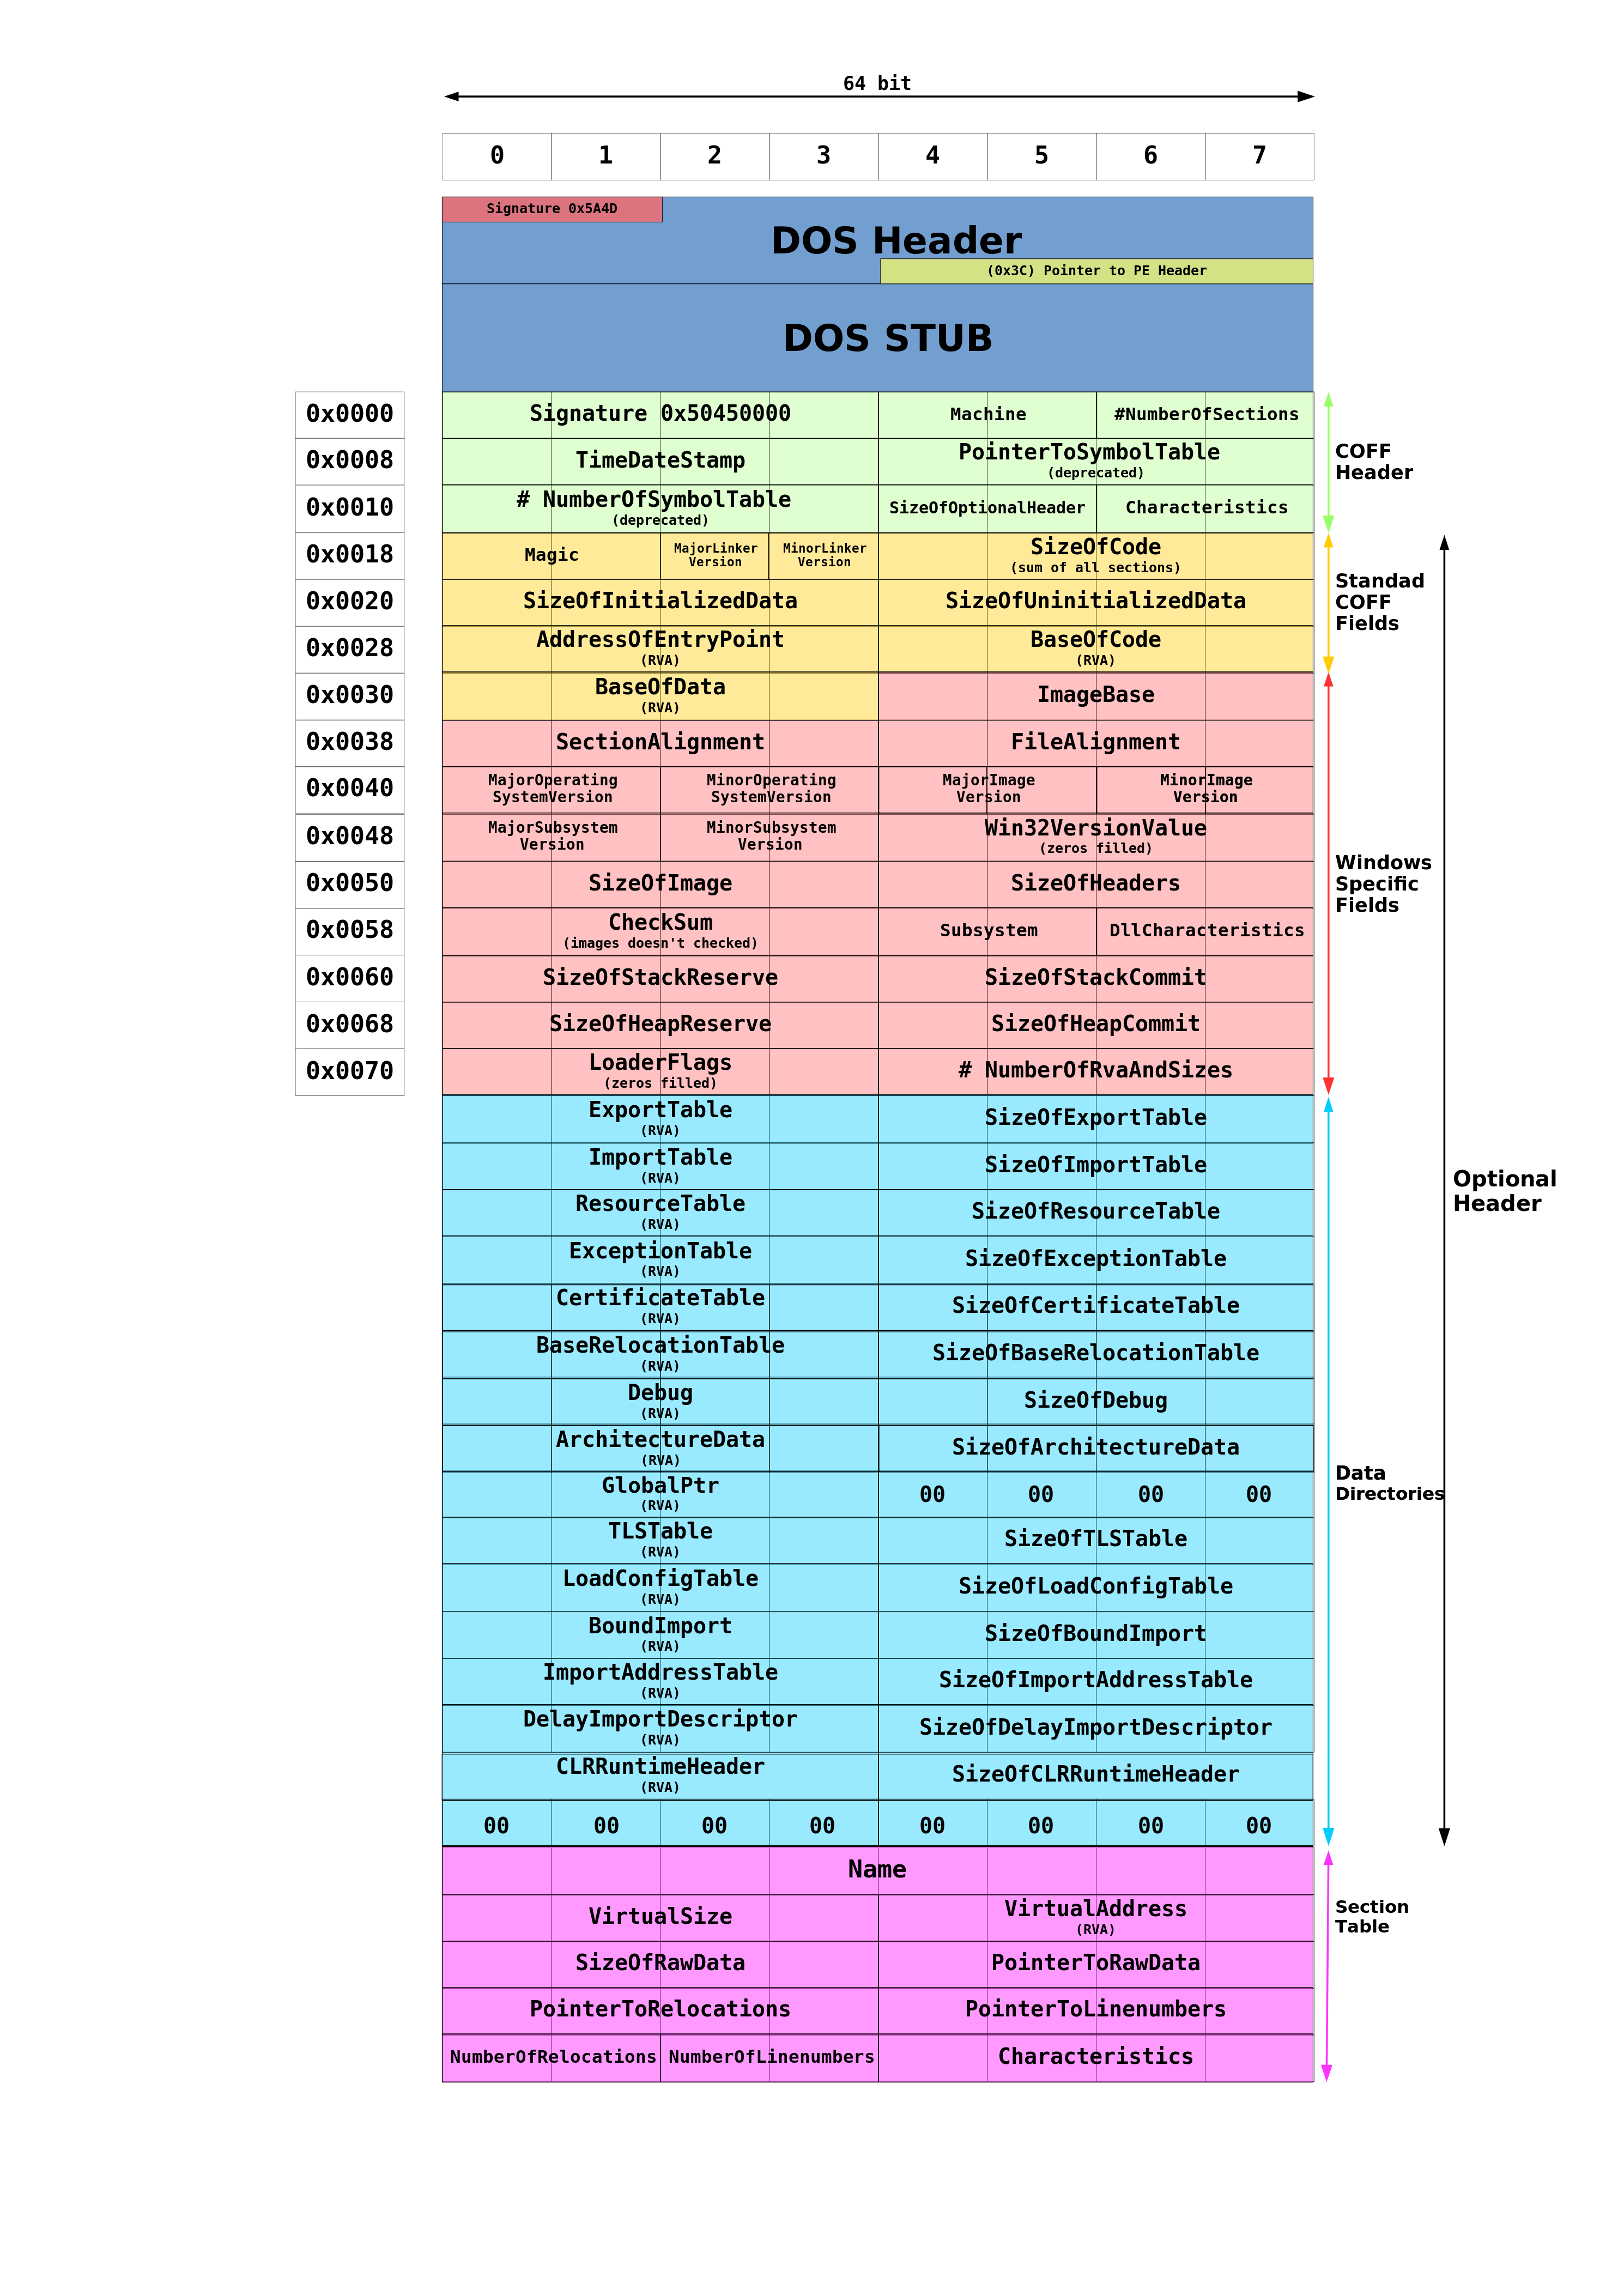
\includegraphics[width=1.0\textwidth]{Portable_Executable_32_bit.png}
\caption{Kết cấu của tệp Portable Executable 32-bit \cite{wikipefile}}
\label{fig:pe32bit}
\end{figure}

Các section của PE chứa code và initialized data mà Windows loader sẽ ánh xạ vào vùng thực thi hoặc vùng bộ nhớ đọc/viết, cũng như là imports, exports, và resources được định nghĩa trong tệp. Mỗi section chưa một header sẽ chỉ định kích cỡ và địa chỉ. Import address table chỉ thị loader function nào sẽ được import tĩnh.Resources section có thể chứa các resource cần thiết cho người dùng như là: cursors, fonts, bitmaps, icons, menus, v.v. Một tập PE cơ bản thường sẽ có \verb|.text| code section và một hoặc nhiều data section (\verb|.data|, \verb|.rdata| hoặc \verb|.bss|). Relocation tables thường được chứa trong \verb|.reloc| section, và được sử dụng bởi Windows loader để reassign base address từ the executable’s preferred base. Section \verb|.tls| thường chứa special thread local storage (TLS) structure cho việc luuaw trữ các biến riêng cho thread. Các section name được gọi ngẫu nhiên từ phía Windows loader, nhưng các tên cụ thể đã được chấp nhận bởi tiền lệ và phổ biến rộng rãi.

\section{Machine Learning}

\subsection{Tổng quan}
\label{ssec:machine-learning-intro}

Trong những năm gần đây, hầu hết các nghiên cứu và tiến bộ sản xuất đều xuất phát từ tiểu ngành cuar Trí tuệ nhân tạo mang tên Machine Learning. Nguyên tắc Machine Learning rất đơn giản; Machine Learning là một phương pháp mà máy tính tìm thấy các pattern từ dữ liệu và đưa các pattern đó vào các ứng dụng. Sau đó, ứng dụng có thể có được thông tin chi tiết về dữ liệu mới dựa trên sự giống nhau với các pattern được xác định \cite{martin2016machine}.

\begin{figure}[htbp!] 
\centering    
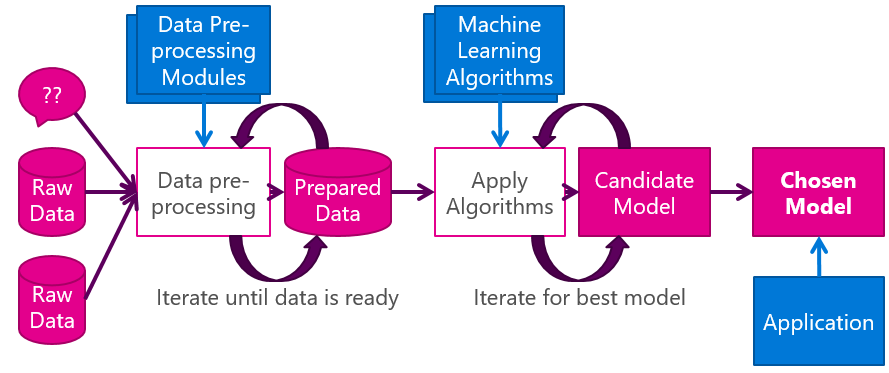
\includegraphics[width=1.0\textwidth]{MLProcess.png}
\caption{Quy trình học máy \cite{martin2016machine}}
\label{fig:ml-process}
\end{figure}

Hãy xem xet các công việc chung (Hình \ref{fig:ml-process}) của một quy trình học máy:

\begin{itemize}
\item Mục tiêu chính của quá trình này là xác định một mô hình. 
Mô hình là điều chính mà ứng dụng có thể gửi yêu cầu để có được thông tin chi tiết về dữ liệu mới.
\item Trước khi đi vào thử nghiệm Machine Learning, chúng ta phải xác định mục đích và cách đánh giá kết quả.
\item Quá trình bắt đầu với việc chuẩn bị dữ liệu. 
Dữ liệu được chuẩn bị là một hoặc nhiều tập dữ liệu đã được xử lý trước (định dạng, làm sạch và lấy mẫu) để sẵn sàng áp dụng thuật toán Machine Learning. 
Chuẩn bị dữ liệu có nghĩa là làm cho dữ liệu có hình dạng tốt nhất để rút ra kết luận khoa học.
\item Bước tiếp theo là áp dụng một hoặc nhiều thuật toán Máy học tạo ra một Mô hình, đó là một quá trình lặp lại và chúng ta có thể lặp lại việc kiểm tra các thuật toán khác nhau cho đến khi chúng ta đạt được một mô hình đủ để đạt được mục đích.
\end{itemize}

Không phải tất cả các vấn đề đều là có thể áp dụng giải pháp học máy. 
Vấn đề này phải là một vấn đề có thể được giải quyết bằng dữ liệu, và có đủ số lượng dữ liệu có liên quan để được sử dụng. 
Như chúng ta sẽ thấy, nhiều vấn đề bảo mật phù hợp với yêu cầu này cực kỳ tốt.

\subsection{Supervised Learning}
\label{ssec:supervised-learning}

Các thuật toán học được giám sát (supervised learning) đưa ra dự đoán dựa trên một tập hợp mẫu, ví dụ: giá cổ phiếu trong lịch sử có thể được sử dụng để đoán giá tương lai.
Thuật toán học được giám sát tìm kiếm các pattern trong dữ liệu được gắn nhãn.
Nó có thể sử dụng bất kỳ thông tin nào có thể có liên quan và mỗi thuật toán sẽ tìm các loại pattern khác nhau.
Sau khi thuật toán đã phát hiện pattern tốt nhất có thể, nó sử dụng pattern đó để đưa ra các dự đoán cho dữ liệu không được dán nhãn.

Khi dữ liệu đang được sử dụng để dự đoán danh mục, học tập được giám sát được gọi là phân loại, ví dụ: chỉ định hình ảnh làm hình ảnh của chú mèo hoặc chó. Khi chỉ có hai lựa chọn, nó được gọi là phân loại hai lớp, nhị thức hoặc nhị phân. Khi có nhiều danh mục hơn, vấn đề này được gọi là phân loại nhiều lớp.

\subsection{Feature Extraction}

Như đã đề cập trong phần \ref{ssec:machine-learning-intro},chúng ta nên trích xuất các thuộc tính từ dữ liệu đầu vào để chúng ta có thể đưa nó vào thuật toán. Ví dụ, trong các trường hợp hình ảnh, dữ liệu có thể được biểu diễn dưới dạng giá trị RGB của mỗi pixel.

Các thuộc tính như vậy được gọi là \textbf{các đặc trưng}, và ma trận được gọi là vector đặc trưng. Quá trình trích xuất đặc trưng từ các tệp gọi là feature extraction. Mục đích của việc feature extraction là để có được một tập hợp dữ liệu nhiều thông tin và không dư thừa.

Các đặc trưng phải thể hiện thông tin cần thiết và có liên quan về tập dữ liệu của chúng ta vì chúng ta không thể đưa ra dự đoán chính xác mà không có nó.
Đó là lí do tại sao feature extraction thường là một nhiệm vụ không rõ ràng và phụ thuộc vào lĩnh vực cụ thể, đòi hỏi nhiều thử nghiệm và nghiên cứu.

Một yêu cầu quan trọng khác đối với một bộ đặc trưng phù hợp là không dư thừa.
Việc xuất hiện các đặc trưng dư thừa, cụ thể là các yếu tố nằm ngoài vùng thông tin hoặc các yếu tố không liên quan, có thể làm cho thuật toán thiên vị, theo đó là việc cung cấp kết quả không chính xác.

\subsection{Classification, Regression và Thresholding}

\textbf{Classification} là công việc xấp xỉ hàm ánh xạ ($f$) từ các biến đầu vào ($X$) để đưa ra biến đầu ra rời rạc ($y$). 
Các biến đầu ra thường được gọi là nhãn hoặc danh mục. 
Hàm ánh xạ dự đoán lớp hoặc nhóm cho một quan sát đã cho.
Ví dụ: một email có thể được phân loại là thuộc một trong hai loại: "spam" và "không phải spam".

\textbf{Regression} là công việc xấp xỉ hàm ánh xạ ($f$) từ các biến đầu vào ($X$) để đưa ra biến đầu ra liên tục ($y$). 
Biến đầu ra là giá trị thực, chẳng hạn như giá trị số nguyên hoặc số thực.
Đây thường là số định lượng, chẳng hạn như số lượng và kích cỡ.
Ví dụ: một căn nhà có thể được dự đoán sẽ bán cho một giá trị đô la cụ thể, có thể trong phạm vi từ 100,000 đô la đến 200.000 đô la.

Các vấn đề classification thường khác các vấn đề regression.
Classification là công việc dự đoán nhãn lớp rời rạc, còn regression là công việc dự đoán số lượng liên tục. 
Tuy nhiên, có một số chồng chéo giữa các thuật toán để phân loại và hồi quy.
Ví dụ, chúng ta có thể sử dụng xác suất, được trả về từ regression, trực tiếp hoặc chuyển nó thành một giá trị nhị phân. 
Để ánh xạ một giá trị logistic regression sang danh mục nhị phân, chúng ta phải định nghĩa một \textbf{classification threshold} (còn gọi là decision threshold).
Có thể giả định rằng classification threshold luôn là 0,5, nhưng threshold phụ thuộc vào các vấn đề cụ thể và do đó đây là giá trị mà chúng ta phải điều chỉnh.

\subsection{Ensemble, Bagging và Boosting}

Khi chúng ta cố gắng dự đoán biến mục tiêu sử dụng bất kỳ phương pháp học máy nào, nguyên nhân hàng đầu của sự khác biệt trong giá trị ban đầu và được dự đoán là noise, variance, và bias. Ensemble giúp giảm hai yếu tố phía sau.

Một ensemble là một tập hợp các mô hình dự đoán để cùng đưa ra dự đoán cuối cùng. Lý do chính là nhiều mô hình dự đoán khác nhau cố gắng dự đoán cùng một biến mục tiêu sẽ thực hiện một công việc tốt hơn so với bất kỳ một đơn lẻ nào. Kỹ thuật ensemble được phân loại thêm vào Bagging và Boosting.

Bagging là một kỹ thuật ensemble đơn giản bằng cách xây dựng nhiều mô hình độc lập và kết hợp chúng bằng những phương pháp lấy trung bình (ví dụ như, lấy trọng số trung bình, đa số phiếu bình chọn hoặc lấy trung bình bình thường). Chúng tôi thường sử dụng tập nhỏ ngẫu nhiên của dữ liệu cho mỗi mô hình, để tất cả các mô hình có chút khác biệt với nhau. Mỗi quan sát có cùng xác suất xuất hiện trong tất cả các mô hình. Bởi vì kỹ thuật này dùng nhiều dự báo không tương quan để tạo ra một mô hình cuối cùng, nó làm giảm lỗi bằng cách giảm variance. Một ví dụ nổi tiếng của kỹ thuật bagging ensemble là Random Forest (được đề cập ở phần \ref{ssec:random-forest}).

Boosting là một kỹ thuật ensemble technique mà các mô hình được xây dựng một cách tuần tự. Kỹ thuật này áp dụng logic trong đó mô hình dự báo phía sa học hỏi từ những sai lầm của những mô hình trước đó. Theo đó, các quan sát có xác suất không đồng đều xuất hiện trong các mô hình tiếp theo. Mô hình dự báo có thể chọn từ nhiều thuật toán như decision trees, regressors, classifiers, v.v. Bởi vì các mô hình phía sau học tập từ những lỗi sai của mô hình phía trước, nó sử dụng ít số iteration để đạt được độ chính xác đã có. Những chúng ta phải chọn điểm dừng phù hợp, hoặc nó có thể dẫn đến việc overfitting trên tập dữ liệu huấn luyện. Gradient Boosting Decision Tree, được đề cập trong phần \ref{ssec:gbdt}, là một ví dụ của kỹ thuật này.

\section{Các phương pháp Machine Learning}

\subsection{Decision Tree}
\label{ssec:decision-tree}

Ngay từ tên của thuật toán, cây quyết định là cấu trúc dữ liệu có cấu trúc của cây. Bộ dữ liệu đào tạo được sử dụng để tạo ra cây, cây này được sử dụng để đưa ra các dự đoán về dữ liệu thử nghiệm. Trong thuật toán này, mục đích là đạt được kết quả chính xác nhất với số lượng ít nhất các quyết định phải được đưa ra. Chúng ta có thể sử dụng cây quyết định có thể cho cả vấn đề phân loại và hồi quy. Bảng \ref{table:decision-tree} đưa ra một ví dụ.

\begin{table}[h]
\caption{Một ví dụ về Decision Tree}
\centering
\label{table:decision-tree}
\begin{tabular}{c l l c c c c}
\hline
Id & Name                       & Sex    & Age  & SibSp & Survived \\	
\hline
1  & Braund, Mr. Owen Harris    & male   & 22.0	& 1     & 0	\\
2  & Cumings, Mrs. John Bradley & female & 38.0	& 1     & 1	\\
3  & Heikkinen, Miss. Laina	    & female & 26.0	& 0     & 1 \\
...& ...                        & ...    & ...  & ...   & ... \\ 
\hline 
\end{tabular}
\end{table}

\begin{figure}[htbp!] 
\centering    
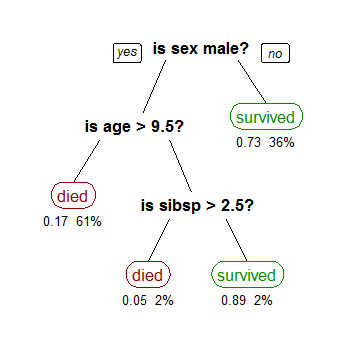
\includegraphics[width=0.5\textwidth]{decesion_tree.png}
\caption{Một ví dụ về Decision Tree \cite{wikidecesiontree}}
\label{fig:decision-tree}
\end{figure}

Trong Hình \ref{fig:decision-tree}, mô hình được đào tạo dựa trên tập dữ liệu và bây giờ có thể phân loại hành khách trong Titanic là sống sót hay không. Cây bao gồm các nút quyết định và các nút lá, và các nút quyết định có thể có nhiều nhánh dẫn đến các nút lá. Nút lá đại diện cho các quyết định hoặc phân loại. Nút đầu tiên đầu tiên được gọi là nút gốc.

Phương pháp cây quyết định đã trở nên phổ biến vì tính đơn giản của nó. Nó có thể xử lý tốt với các bộ dữ liệu lớn và có thể xử lý nhiễu trong bộ dữ liệu rất tốt. Một ưu điểm khác là không giống như các thuật toán khác, chẳng hạn như SVM hoặc KNN, cây quyết định hoạt động trong một hộp màu trắng, có nghĩa là chúng ta có thể thấy kết quả thu được như thế nào và quyết định nào dẫn đến nó.

\subsection{Random Forest}
\label{ssec:random-forest}

Random Forest là một trong những thuật toán học máy phổ biến nhất. Nó hầu như không có đòi hỏi việc chuẩn bị dữ liệu và mô hình hóa nhưng thường kết thúc trong các kết quả không chính xác. Random Forests dựa trên các cây quyết định được mô tả trong phần trước \ref{ssec:decision-tree}. Cụ thể hơn, Random Forest là tập hợp các cây quyết định, tạo ra độ chính xác dự đoán tốt hơn. Đó là lí do tại sao nó được gọi là rừng - nó là bộ cây quyết định.

Ý tưởng thiết yếu là phát triển nhiều cây quyết định dựa trên các tập con độc lập của tập dữ liệu. Ở mỗi nút, \textit{n variables} trong số các tính năng được chọn ngẫu nhiên, và phân chia tốt nhất trên các biến này được sử dụng.

Chúng ta có thể mô tả thuật toán như sau \cite{biau2012analysis}:

\begin{enumerate}
\item Nhiều cây được xây dựng trên khoảng hai phần ba số liệu huấn luyện một cách ngẫu nhiên.
\item Một số biến được chọn ngẫu nhiên trong số tất cả các biến dự báo. Sau đó, sự phân chia tốt nhất trên những cái này được sử dụng để chia nút. Theo mặc định, số lượng các biến được chọn là căn bậc hai của tổng số của tất cả các dự đoán, và nó là hằng số cho tất cả các cây.
\item Với phần còn lại của dữ liệu, tỷ lệ phân loại sai được tính toán. Tổng tỷ lệ lỗi được tính là overall out-of-bag error rate.
\item Mỗi cây được đào tạo cho kết quả phân loại của nó và lớp được nhận điểm cao nhất được chọn là kết quả.
\end{enumerate}

Vì chúng ta đang sử dụng nhiều cây quyết định, thuật toán này loại bỏ việc feature selection để xóa các tính năng không cần thiết - chúng sẽ không được tính đến trong mọi trường hợp. Nhu cầu duy nhất cho feature selection với các thuật toán random forest phát sinh khi có nhu cầu giảm số lượng các đặc trưng. Hơn thế nữa, out-of-bag error rate được coi là phương pháp xác thực chéo của thuật toán. Điều này loại bỏ nhu cầu về các biện pháp xác thực chéo, mà sẽ phải được thực hiện nếu sử dụng phương pháp khác \cite{mitchell1997machine}.

Random forest thừa hưởng nhiều ưu điểm của thuật toán cây quyết định. 
Chúng phù hợp cho cả vấn đề hồi quy và phân loại, chúng dễ tính toán và huấn luyện nhanh chóng để phù hợp. 
Nó cũng thường xuyên dẫn đến độ chính xác tốt hơn.
Tuy nhiên, không giống như cây quyết định, nó không phải là rất dễ dàng để giải thích kết quả.
Trong cây quyết định, bằng cách kiểm tra cây kết quả, chúng ta có thể thu được thông tin giá trị về các biến nào có liên quan và chúng ảnh hưởng như thế nào đến kết quả.
Random forest cũng có thể được mô tả như một thuật toán vững chắc hơn so với cây quyết định vì nó là sự kết hợp của nhiều cây quyết định \cite{louppe2014understanding}.

\subsection{Gradient Boosting Decision Trees}
\label{ssec:gbdt}

Gradient Boosting Decision Tree (GDBT) is an ensemble model of decision trees, which are trained in sequence \cite{friedman2001greedy}. 
In each iteration, GBDT learns the decision trees by fitting the negative gradients (also known as residual errors).
The main cost in GBDT lies in learning the decision trees, and the most time-consuming part of learning a decision tree is to find the best split points.
One of the most common algorithms to find split points is the pre-sorted algorithm \cite{mehta1996sliq, shafer1996sprint}, which lists all possible split points on the pre-sorted feature values. 
This algorithm is simple and can find the optimal split points.
However, it is wasteful in both training speed and memory consumption. Another famous algorithm is the histogram-based
algorithm \cite{ranka1998clouds, jin2003communication, li2008mcrank}. 
Instead of finding the split points on the sorted feature values, histogram-based algorithm buckets continuous feature values into discrete bins and uses these bins to construct feature histograms during training.

\bigskip
\begin{algorithm}[H]
 \KwData{$I$: training data, $d$: max depth}
 \KwData{$m$: feature dimension}
 $nodeSet \leftarrow \{0\} \triangleright$ tree nodes in current level \\
 $rowSet \leftarrow \{\{0, 1, 2, ...\}\} \triangleright$ data indices in tree nodes \\
 \For{$i = 1$ \KwTo $d$}{
  \For{$node$ \textbf{in} $nodeSet$}{
    $usedRows \leftarrow rowSet[node]$ \\
    \For{$k = 1$ \KwTo $m$}{
      $H \leftarrow$ new Histogram() \\
      $\triangleright$ Build histogram \\
      \For{$j$ \textbf{in} $usedRows$}{
        bin $\leftarrow$ I.f[k][j].bin \\
        H[bin].y $\leftarrow$ H[bin].y + I.y[j] \\
        H[bin].n $\leftarrow$ H[bin].n + 1
      }
    }
  }
  Update $rowSet$ and $nodeSet$ according to the best split points
 }
 \caption{Histogram-based Algorithm}
 \label{alg:histogram-based}
\end{algorithm}
\bigskip

As shown in Algorithm \ref{alg:histogram-based}, the histogram-based algorithm finds the best split points based on the feature histograms. 
It costs $O(\#data \times \#feature)$ for building histogram and $O(\#bin \times \#feature)$ for finding the split point. Since $\#bin$ is usually much smaller than $\#data$, histogram building will control the computational complexity. If we can reduce $\#data$ or $\#feature$, we will be able to speed up the training of GBDT extensively.

\subsection{Support Vector Machine}

Support Vector Machines (SVM) is another machine learning algorithm that is commonly used for classification problems. The main idea relies on finding such a hyperplane, that would separate the classes in the best way. The term "support vectors" refers to the points lying closest to the hyperplane, that would change the hyperplane position if removed. The distance between the support vector and the hyperplane is referred to as margin.

Intuitively, we know that the further from the hyperplane our groups lie, the more accurate predictions we can get. That is why, although multiple hyperplanes can be found, the goal of the SVM algorithm is to find such a hyperplane that would result in the maximum margins.

SVMs are usually able to produce good accuracy, particularly on clean datasets. 
Further, it is good at working with the high-dimensional datasets, also when the number of dimensions is higher than the number of the samples. 
Additionally, for large datasets with a lot of noise or overlapping classes, it can be more effective.
However, with more massive datasets training time can be extended \cite{jing2010view}.

\subsection{K-Nearest Neighbors}

The k-Nearest Neighbors algorithm (k-NN) is a non-parametric method used for classification and regression. 
The k-NN does not make any assumptions about the data structure, which makes it become a good solution in the real world where most of the data does not follow the typical theoretical assumptions. 
K-NN is also a lazy algorithm, which means there is no specific training phase or it is very insignificant. 
Also, lack of generalization means that k-NN keeps all the training data, i.e., the most the training data is required during the testing phase.

The algorithm is based on feature similarity. 
How closely out-of-sample features match the training set determines how k-NN classify a given data point.
The Euclidean Distance,  which is defined by the formula below, is the most used method for continuous variables in k-NN.

\begin{center}
$EuclideanDistance =  \sqrt{ \sum_{i=1}^{n}(q_i - p_i)^2 }$
\end{center}

The drawback of the k-NN algorithm is the lousy performance on the unevenly distributed datasets. 
Hence, if one class hugely overshadows the other ones, it is more likely to have more neighbors of that class due to their large number, and therefore, make incorrect predictions \cite{laaksonen1996classification}.

\subsection{Neural Networks}

\subsubsection{Overview}

The idea behind neural networks, i.e., having computational units that produce “intelligent” results only through interactions with each other, was inspired by the brain. 
For instance, the Neocognitron system, proposed by Kunihiko Fukushima in 1980, took inspiration from the mammalian visual system and laid the foundation for modern convolutional networks \cite{goodfellow2016deep}. 
Hence, the artificial neurons in these networks mimic the structure of biological ones. 

The very first artificial model of the biological neuron is in fact perceptron, introduced by Frank Rosenblatt in 1958 \cite{rosenblatt1958perceptron}. 
Perceptron is an algorithm for supervised learning in machine learning. Perceptron, in essence, is a simple function that turns inputs (usually a real-valued vector) into one binary output.

\begin{figure}[htbp!] 
\centering    
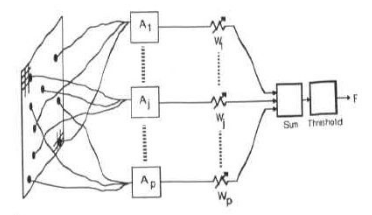
\includegraphics[width=0.5\textwidth]{perceptron.png}
\caption{Basic structure of a perceptron \cite{minsky1969perceptron}}
\label{fig:perceptron}
\end{figure}

Following Figure \ref{fig:perceptron}, we can see the perceptron receives \textit{p} inputs, $A_1$, $A_2$, ..., $A_p$ (or $x_1$, $x_2$, ..., $x_p$, depending on the source. 
The inputs are then respectively weighted by $w_1$, $w_2$, ..., $w_p$, which are real numbers indicating the importance of each of the input values. The output \textit{F} will then be calculated using the sum of those weighted inputs. 
Additionally, because the output is a binary value, a threshold is used to achieve the desired result. To be more specific, a perceptron is written as follows:

\begin{center}
$F = \begin{cases}
1 & if \sum_{i}^{p} A_i w_i \geq Threshold \\
0 & if \sum_{i}^{p} A_i w_i < Threshold
\end{cases}$
\end{center}

Consequently, the output of a perceptron is controlled by two things: the weights $w_1$, $w_2$, ..., $w_p$ and the Threshold. 
In modern neuron networks, however, the equation changed a bit by bringing the Threshold to the other side of the inequalities. 
The additive inverse of Threshold is then known as Bias, and the perception will be rewritten as:

\begin{center}
$F = \begin{cases}
1 & if \sum_{i}^{p} A_i w_i + Bias \geq 0 \\
0 & if \sum_{i}^{p} A_i w_i + Bias < 0
\end{cases}$
\end{center}

\subsubsection{Activation function}

Perceptron is the precursor to modern artificial neurons. Instead of returning only a binary output, an artificial neuron now produces values that are anywhere in the range [0,1]. 
The reason is to help in the learning process of a network. Neural networks can learn, i.e., finding the appropriate weights and biases given sufficient input data. 
The learning process, however, needs to be progressive, which means weights and biases get increasingly close to the "good" values. 
Having a binary output for each of the neurons makes it hard for this process to be done. 
For training a neural network, we use an error function to see how far or close the network is to the optimal results.
Because of the binary output of perception, a small change in the network's parameters can lead to a stark difference for the output, making it hard to tune the parameters to achieve a good result. 
Therefore, modifications must be made to the original perceptron model. 
Instead of using 0 as the threshold at which signals are allowed to be fired, we can use an activation function to map the output to the range we need appropriately.

\begin{figure}[htbp!] 
\centering    
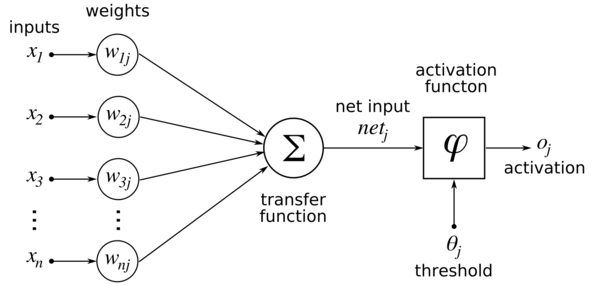
\includegraphics[width=0.7\textwidth]{artificial_neuron.png}
\caption{Structure of an artificial neuron \cite{wikian}}
\label{fig:artificial-neuron}
\end{figure}

The activation function takes as input the weighted sum of the input values fed to the perceptron and returns a value in the range [0,1]. 
Historically, the Sigmoid function was used for this purpose as it can squash the sum to the desired range \cite{li2015cs231n}. 
Modern networks, however, use different functions as well, such as hyperbolic tan function (tanh) or rectified linear unit (ReLU), to achieve better performance \cite{li2015cs231n}.

\subsubsection{Feedforward and Backpropagation}

Two operations are particularly important in neural networks: Feedforward and Backpropagation.

Feedforward is used in both the training and testing stage of a network. 
The task we need to do in feedforward is straightforward: Passing output of a layer as the input of the next layer.
Since all we are doing is unidirectionally putting values through the network from the input layer to the output layer, the operation is called feedforward. 

Backpropagation is generally used in the training stage to help neural networks learn their parameters, and it is considered an optimization. 
Different from feedforward, the job of this operation is to propagate error of the output values back to the network to update the network parameters. 
Backpropagation works by first do the normal feedforward operation on the network with the given input. 
After the output is obtained, we compare the output to the desired output, using a loss function to generate an error term for each of the neuron in the output layer. 
The error values are then propagated backward from the output layer until every neuron receive their respective error term. 
The error terms will be used to calculate the gradient, with which we can update the weights of the network to minimize the loss function as the process repeats. 
To find the most fitting parameters, gradient descend algorithm is usually applied.

\section{Classification Metrics}

In this section, we review how to use several common metrics that are used to evaluate predictions for classification problems.

\subsection{Logarithmic Loss}

Logarithmic loss, or log-loss for short, is a performance metric for evaluating the predictions of probabilities of membership to a given class.

Log-loss takes into account the uncertainty of your prediction based on how much it varies from the actual label, which gives us a more nuanced view of the performance of our model.
In binary classification, with $y$ is a binary indicator (0 or 1) of whether class label $c $is the correct classification and $p$ is the model predicted probability, the formula equals:

\bigskip
\begin{center}
    $LogLoss = -(y\log(p) + (1 - y)\log(1 - p))$
\end{center}
\bigskip

The scalar probability between 0 and 1 can be seen as a measure of confidence for a prediction by an algorithm.
Smaller log-loss is better with 0 representing a perfect log-loss.

\subsection{Confusion Matrix}
\label{ssec:confusion_matrix}

\begin{figure}[H]
    \centering    
    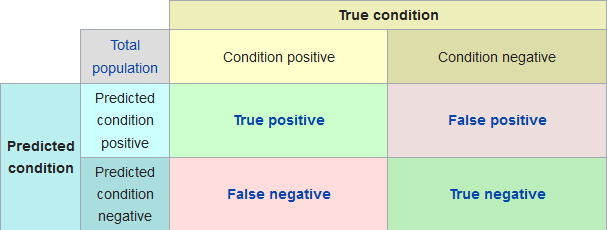
\includegraphics[width=0.7\textwidth]{confusion_matrix.png}
    \caption{Confusion matrix \cite{wiki_confusion_matrix}}
    \label{fig:confusion_matrix}
\end{figure}

A clean and unambiguous way to show the prediction results of a classifier is to use a confusion matrix (also called a contingency table).
For a binary classification problem, the table has two rows and two columns (which is shown in Figure \ref{fig:confusion_matrix}). 
Across the top is the actual class labels and down the side are the predicted class labels. 
Each cell carries the number of predictions made by the classifier that fall into that cell.

\begin{figure}[H]
    \centering    
    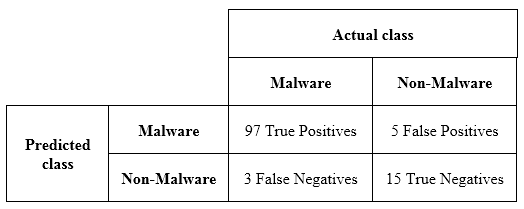
\includegraphics[width=0.7\textwidth]{confusion_matrix_example.png}
    \caption{An example of confusion matrix}
    \label{fig:confusion_matrix_example}
\end{figure}

Figure \ref{fig:confusion_matrix_example} is an example of binary classification in malware detection. 
Some of the input files are malware, and our test correctly says they are positive. 
They are called true positives (TP). 
In contrast, some are malware, but the test incorrectly claims they are not. 
They are called false negatives (FN). 
Some are clean files, and the test says they are not malware – true negatives (TN). 
Finally, there might be clean files have a positive test result – false positives (FP).

There are many derived ratios from confusion matrix, and the most common ones are listed below:

\begin{itemize}
    \item True Positive Rate (TPR), eqv. with hit rate, recall: $TPR = TP/P = TP/(TP + FN)$
    \item True Negative Rate (TNR): $SPC = TN/N = TN/(TP + FN)$
    \item Precision or Positive Predictive Value (PPV): $PPV = TP/(TP + FP)$
    \item Negative Predictive Value (NPV): $NPV = TN/(TN + FN)$
    \item Fall-out or False Positive Rate (FPR): $FPR = FP/N = FP/(TP + FN) = 1 - TNR$
    \item False Discovery Rate (FDR): $FDR = FN/(FN + TP) = 1 - PPV$
    \item Miss Rate or False Negative Rate (FNR): $FNR = FN/(FN + TP) = 1 - TPR$
\end{itemize}

\subsection{Overall Accuracy}

Overall accuracy is the number of correct predictions made as a ratio of all predictions made.

\begin{center}
    ${Accuracy} =  \cfrac{True\ positive + True\ negative}{Condition\ positive + Condition\ negative}$
\end{center}

Overall Accuracy essentially tells us out of all of the reference sites what proportion were mapped correctly. 
The overall accuracy is usually expressed as a percent, with 100\% accuracy being a perfect classification where all reference site were classified correctly. 
Overall accuracy is the easiest to calculate and understand but ultimately only provides the map user and producer with necessary accuracy information.

This is the most common evaluation metric for classification problems, it is also the most misused. 
It is only suitable when there is an equal number of observations in each class (which is rarely the case) and that all predictions and prediction errors are equally important (which is often not the case).

\subsection{Precision and Recall}

Precision can be thought of as a measure of a classifiers exactness. Precision attempts to answer the question "What proportion of positive identifications was actually correct?". A low precision can also indicate a large number of False Positives.

\begin{center}
    ${Precision} =  \cfrac{True\ positive}{True\ positive + False\ positive}$
\end{center}

Recall is the number of True Positives divided by the number of True Positives and the number of False Negatives. Computing in another way is the number of positive predictions divided by the number of positive class values in the test data. Recall attempts to answer "What proportion of actual positives was identified correctly?". It is also called Sensitivity or the True Positive Rate.

\begin{center}
    ${Recall} =  \cfrac{\sum True\ positive}{\sum Condition\ positive}$
\end{center}

\subsection{Area Under ROC curve}
\label{ssec:auroc}

Area Under the Receiver Operating Characteristic curve, AUROC or AUC for short, is a performance metric for binary classification problems. The AUROC has several equivalent interpretations:

\begin{itemize}
\item The expectation that a uniformly drawn random positive is ranked before a uniformly drawn random negative.
\item The expected proportion of positives ranked before a uniformly drawn random negative.
\item The expected true positive rate if the ranking is split just before a uniformly drawn random negative.
\item  The expected proportion of negatives ranked after a uniformly drawn random positive.
\item  The expected false positive rate if the ranking is split just after a uniformly drawn random positive.
\end{itemize}

An area of $1.0$ represents a model that made all predictions perfectly. A rough guide for classifying the accuracy of a classification test is the typical academic point system: 

\begin{itemize}
\item 0.9 - 1.0 = Excellent
\item 0.8 - 0.9 = Good
\item 0.7 - 0.8 = Fair
\item 0.6 - 0.7 = Poor
\item 0.5 - 0.6 = Fail
\end{itemize}

\subsubsection{Compute the AUROC}

Assume we have a binary classifier such as logistic regression. First, we compute two metrics from the confusion matrix (their formula are mentioned in section \ref{ssec:confusion_matrix}), which will be later combined into one:

\begin{enumerate}
    \item \textbf{True positive rate (TPR).} Intuitively this metric agrees to the proportion of positive data points that are correctly considered as positive, with respect to all positive data points. In other words, the higher TPR, the fewer positive data points we will miss.
    \item \textbf{False positive rate (FPR).} This metric corresponds to the proportion of negative data points that are mistakenly considered as positive, concerning all negative data points. In other words, the higher FPR, the more negative data points will be misclassified.
\end{enumerate}

\begin{figure}[H]
    \centering    
    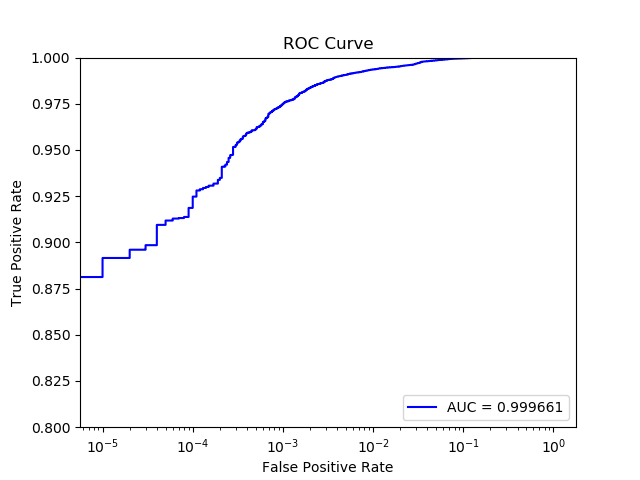
\includegraphics[width=0.8\textwidth]{roc_curve.png}
    \caption{An example of Receiver Operating Characteristic curve}
    \label{fig:auroc}
\end{figure}

Then, we combine the FPR and the TPR into one single metric by computing the two former metrics with many different threshold (for example, 0.00, $10^-5$, $10^-4$, $10^-3$, ..., 1.00, as shown as in Figure \ref{fig:auroc}) for the logistic regression, then plot them on a single graph, with the FPR values on the x-axis and the TPR values on the y-axis. The resulting curve is called  Receiver Operating Characteristic curve, and the metric we consider is the area under this curve.

\section{LightGBM - A Gradient Boosting Framework}

LightGBM, which means Light Gradient Boosting Machine, is a gradient boosting framework that uses tree-based learning algorithm \cite{ke2017lightgbm}. This framework is obtaining an extreme reputation due to its following advantages:

\begin{itemize}
\item Faster training speed and higher efficiency
\item Lower-memory usage
\item Better accuracy
\item Parallel and GPU learning supported
\item Capable of handling the large-scale data
\end{itemize}

The framework uses two following techniques to solve problems when the feature dimension is high, and data size is considerable: Gradient-based One-Side Sampling and Exclusive Feature Bundling.

\subsection{Gradient-based One-Side Sampling}

Base on the notice that, while there is no weight for data instance in the gradient-boosting decision tree, data instances with different gradients play different roles in the computation of information gain. 
In particular, according to the definition of information gain, instances with larger gradients (i.e., under-trained instances) will contribute more to the information gain.
Since, when subsampling the data instances, to retain the accuracy of information gain estimation, LightGBM tends to keep instances with large gradients (e.g., larger than a pre-defined threshold, or among the top percentiles), and only randomly drops instances with small gradients.
They proved that such a treatment could lead to a more accurate gain estimation than uniformly random sampling, with the same target sampling rate, especially when the value of information gain has a vast range.

\subsection{Exclusive Feature Bundling}

Regularly in real applications, although there are a large number of features, the feature space is quite sparse, which provides the LightGBM a possibility of using a nearly lossless approach to reduce the number of active features.
In fact, in a sparse feature space, many features are almost exclusive, i.e., they rarely take nonzero values together, e.g., the one-hot encoding features, therefore, the framework could safely bundle such unique features.
LightGBM uses an efficient algorithm named Exclusive Feature Bundling, which is a greedy algorithm with a constant approximation ratio.
Specifically, they reduce the optimal bundling problem to a graph coloring problem by taking features as vertices and add edges for every two features if they are not together exclusive.
